\documentclass[a4paper, 12pt]{article}
\usepackage [MeX]{polski}
\usepackage [utf8] {inputenc}
\usepackage {hyperref}
\usepackage{graphicx}
\usepackage[nottoc,numbib]{tocbibind}

\title {Projekt z przedmiotu GIS - sprawozdanie I}
\author{Marek Jasiński, Przemysław Piotrowski}

\begin{document}

\maketitle

\section{Treść zadania}

\paragraph{Temat zadania}
Znajdowanie zbioru najkrótszych ścieżek pomiędzy parą wybranych lub wylosowanych wierzchołków grafu przy awaryjnych krawędziach.

\paragraph{Opis zadania}
Muszą być spełnione następujące warunki: a)pierwsza wygenerowana ścieżka: najkrótsza ścieżka pomiędzy wybraną parą wierzchołków b)każda następna wygenerowana ścieżka posiada krawędź różną od co najmniej jednej krawędzi ścieżki z punktu a) i minimalną długość. Krok b) jest powtarzany kolejno aż do wyczerpania wszystkich krawędzi ścieżki z punktu a) Dane do projektu: G=(V,E) - graf o zadanej strukturze, wylosowana lub wybrana para wierzchołków. Zastosowanie: wyznaczanie ścieżek rezerwowych w sieci w sytuacji awarii pojedynczej krawędzi sieci. Literatura: N.Christofides, Graph Theory - an algorithmic approach, Academic Press 1975, str. 150- 157, 167-170. M.Sysło, N.Deo, J.Kowalik, Algorytmy optymalizacji dyskretnej, PWN 1995. N.Deo, Teoria grafów i jej zastosowania w technice i informatyce. PWN 1980.

\section{Propozycja rozwiązania}

\paragraph{Wejście programu}
Program będzie przyjmował na wejściu graf oraz dwa wierzchołki: źródłowy i~docelowy. Graf będzie grafem nieskierowanym z~ważonymi krawędziami (wagi nieujemne) bez krawędzi równoległych. Graf będzie zadany w~pliku tekstowym. Format tego pliku będzie zgodny z~formatem DOT \cite{dot}. Parametrami programu będą:

\begin{itemize}
\item nazwa pliku tekstowego zawierającego opis grafu w~formacie DOT,
\item nazwa wierzchołka źródłowego (ang. {\it source}) i~nazwa wierzchołka docelowego (ang. {\it target}).
\end{itemize}

Przykładowe wywołanie programu może wyglądać w~ten sposób:

\begin{verbatim}
$ ./ap graph.dot -s w1 -t w5
\end{verbatim}

{\it ap} jest skrótem od {\it Alternate Path} - tak będzie nazywał się nasz program. Przykładowy plik z~zadanym grafem wejściowym może wyglądać~w ten sposób:

\begin{verbatim}
/* graph.dot */
graph G {
	w1 -- w2 [weight=1];
	w2 -- w3 [weight=1];
	w1 -- w4 [weight=1];
	w4 -- w2 [weight=1];
	w2 -- w5 [weight=1];
	w5 -- w3 [weight=1];
}
\end{verbatim}

Plik opisujący graf może być przygotowany ręcznie, zostać pobrany z~Internetu, a~także będzie mógł być wygenerowany przy pomocy naszego drugiego programu, tj. generatora grafów. Opis działania generatora grafów można znaleźć w~paragrafie \ref{generator}.

\paragraph{Przetwarzanie}
Graf będzie wewnętrznie reprezentowany w~postaci listy sąsiedztwa, której implementację dostarcza biblioteka Boost Graph \cite{bgl}. Pomimo, że biblioteka dostarcza implementację algorytmu znajdującego najkrótszą ścieżkę pomiędzy dwoma wierzchołkami, zaimplementujemy własny algorytm oparty na algorytmie Dijkstry. Ogólny algorytm będzie polegał na znalezieniu najkrótszej ścieżki pomiędzy wierzchołkami źródłowym i~docelowym oraz wykorzystaniu jej do dalszego przetwarzania. Kolejne krawędzie z~tej ścieżki będą tymczasowo usuwane, aby uruchamiać algorytm znajdywania najkrótszej ścieżki, który dostarczy alternatywną ścieżkę dla awaryjnej krawędzi. Warto zwrócić uwagę na to, że mogą istnieć krawędzie, których usunięcie spowoduje, że graf przestanie być spójny. Takie krawędzie zostaną oznaczone kolorem czerwonym, jako krytyczne. Nie ma alternatywnych ścieżek w~grafie dla krawędzi krytycznych.

\paragraph{Wyjście programu}
Wizualizację rezultatu działania programu zapewni program NEATO z~pakietu Graphviz \cite{gv}. Służy on do rysowania grafów nieskierowanych. Za pomocą programu NEATO zostaną wygenerowane pliki, na podstawie których zostaną wygenerowane strony HTML. Na stronach będzie można zobaczyć jak wyglądają najkrótsza ścieżka pomiędzy wierzchołkami źródłowym i~docelowym oraz najkrótsze ścieżki alternatywne (po kliknięciu na krawędź, którą uznaje się za awaryjną). Przykładowa zawartość stron może wyglądać w~ten sposób:

\begin{figure}[ht]
\begin{minipage}[b]{0.45\linewidth}
\centering
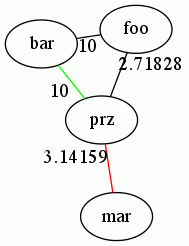
\includegraphics[width=\textwidth]{picture1.png}
\caption{\em Główny obrazek (na stronie index.html)}
\label{fig:picture1}
\end{minipage}
\hspace{0.5cm}
\begin{minipage}[b]{0.45\linewidth}
\centering
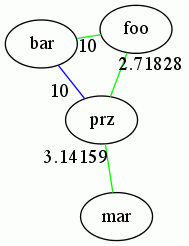
\includegraphics[width=\textwidth]{picture2.png}
\caption{\em Po kliknięciu na zieloną krawędź na głównym obrazku}
\label{fig:picture2}
\end{minipage}
\end{figure}

Na rysunku po lewo widzimy najkrótszą ścieżkę pomiędzy wierzchołkami \texttt{mar} a \texttt{bar}. Została ona oznaczona na kolorowo. Składa się z~dwóch krawędzi. Na wypadek awarii krawędzi zielonej istnieje ścieżka alternatywna, która jest przedstawiona na rysunku po prawo. Czerwona krawędź jest krytyczna - nie ma dla niej alternatywnych ścieżek.

Drugim rezultatem działania programu będzie plik \texttt{report.txt} zawierający informacje o~najkrótszej ścieżce oraz ścieżkach alternatywnych. Przy każdej ze ścieżek będzie informacja o~koszcie (sumie wag). Przykładowa zawartość pliku raportu może wyglądać w~ten sposób:

\begin{verbatim}
Shortest path: mar--prz--bar Cost: 13.1416
mar--prz | No emergency path
prz--bar | mar--prz--foo--bar Cost: 15.8599
\end{verbatim}

\paragraph{Generator grafów}
\label{generator}
Złożoność obliczeniowa programu badana będzie na wygenerowanych grafach pochodzących z generatora grafów. Danymi wyjściowymi generatora będą grafy zapisane w formacie DOT. Grafy te będą odwzorowywać sieci małego świata\cite{amaral2000classes}. Oznacza to, że większość wierzchołków nie sąsiaduje ze sobą, ale pomiędzy większością par wierzchołków można znaleźć ścieżkę składającą się z małej liczby krawędzi. Sieci takie często obserwowane są np. w sieciach społecznościowych. Krawędź oznacza wtedy, że dwie osoby się znają.

Tworzenie przykładowego grafu małego świata składa się z dwóch kroków. Pierwszym z nich jest stworzenie grafu o regularnej strukturze. Przykład zaprezentowany jest na Rys. \ref{fig:regul}. Następnie należy dla każdej z krawędzi wylosować, czy powinna ona zostać przepięta, czy też nienaruszona. W efekcie powstaje graf jak na Rys. \ref{fig:pomiesz}. Dla większej liczby wierzchołków graf widocznie nabiera cech ,,małego świata''.

\begin{figure}[ht]
\begin{minipage}[b]{0.45\linewidth}
\centering
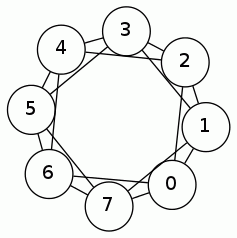
\includegraphics[width=\textwidth]{regularny.png}
\caption{\em Graf o regularnej strukturze}
\label{fig:regul}
\end{minipage}
\hspace{0.5cm}
\begin{minipage}[b]{0.45\linewidth}
\centering
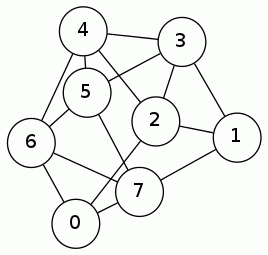
\includegraphics[width=\textwidth]{pomieszany.png}
\caption{\em Graf po przemieszaniu krawędzi}
\label{fig:pomiesz}
\end{minipage}
\end{figure}

Parametrami generatora będą:
\begin{itemize}
\item plik wyjściowy,
\item liczba wierzchołków,
\item liczba krawędzi wychodzących z każdego z wierzchołków,
\item prawdopodobieństwo przepięcia krawędzi.
\end{itemize}

Przykładowe wywołanie:
\begin{verbatim}
$ ./gg graph.dot -n 30 -e 2 -p 0.20
\end{verbatim}

\paragraph{Testy i~eksperymenty}
W celu zbadania złożoności algorytmu stworzony zostanie skrypt zapisujący czas działania programu wraz z długością najkrótszej ścieżki pomiędzy wylosowanymi wierzchołkami. Przykładowy wynik działania prezentuje Rys. \ref{fig:tabela}.

\begin{figure}[ht]
\centering
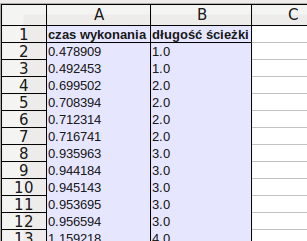
\includegraphics[scale=0.7]{tabela.png}
\caption{\em Zestawienie wynikow}
\label{fig:tabela}
\end{figure}

Dzięki takiemu zestawieniu będzie można sprawdzić, czy złożoność teoretyczna algorytmu została wyznaczona poprawnie.

\begin{thebibliography}{}
\bibitem{dot} ,,The DOT Language'' \\ \url{http://www.graphviz.org/doc/info/lang.html}
\bibitem{bgl} ,,The Boost Graph Library'' \\ \url{http://www.boost.org/doc/libs/1_53_0/libs/graph/doc/index.html}
\bibitem{gv} ,,Graphviz - Graph Visualization Software'' \\ \url{http://www.graphviz.org/}
\bibitem{amaral2000classes} ,,Classes of small-world networks'', Amaral, Lu{\i}s A Nunes and Scala, Antonio and Barth{\'e}l{\'e}my, Marc and Stanley, H Eugene
\end{thebibliography}

\end{document}